\section{Design} \label{sec:design}

\begin{figure}[t!] 
     \centering 
     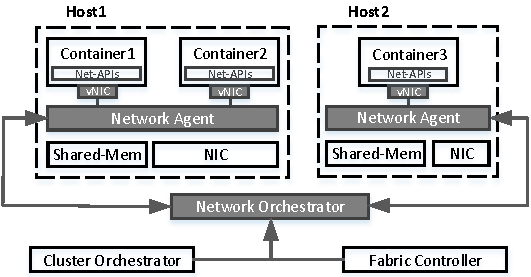
\includegraphics[width=3.2in]{figures/system-arch.pdf} 
    \caption{\label{fig:sysarch} The overall system architecture of~\sysname. Gray boxes are building blocks of~\sysname.} 
\end{figure} 

This section presents the high-level design of \sysname. We introduce
the requirements and concerns in the designs of control-plane, data-plane
and network access layer, and explain what design choices \sysname makes 
and what the reasons are behind these design choices.

\subsection{Overview}

Our goal is to design a complete network solution which can enable containers
to communicate with portability, isolation and high performance at the same time.
Basically, this solution has three major components: control-plane, data-plane 
and networking abstraction. 

A \textbf{control-plane} handles IP address assignment, routing and manages global states of a container network.
A flexible control-plane is a must for portability and isolation. 
It should permit a container to register its own IP address in the network
from any host; It also should automatically configure and update the routing 
to each container. One unique requirement for \sysname's control-plane,
compared with existing container networking solutions, is to be able to 
select data-plane (e.g. shared-memory, RDMA, TCP/IP, etc.) in real-time
according to multiple factors, such as container locations, hardware 
capabilities and so on. 
There are several routing schemes that are used by existing
container networking solutions, and they are optional for \sysname. 
For example, Calico and WeaveNet build distributed routing scheme on top of 
distributed routing protocols (e.g. BGP), while Docker default overlay network
and DaoliNet use centralized routing planes based on OpenFlow and OVS.

A \textbf{data-plane} delivers data from sender containers to receiver 
containers. \sysname's data-plane should always achieve a good trade-off
between isolation, portability and performance. 
As introduced in \S\ref{sec:motivation}, there are many data-plane mechanisms
for two containers, such as shared-memory (intro-host), TCP/IP, DPDK, RDMA, etc..
Different mechanisms have different properties on portability, isolation and 
performance. Therefore, we need to decide is to choose a single mechanism, or
integrate multiple mechanisms together.

A \textbf{network abstraction} defines how containers access the networks
provided by \sysname. Application inside containers are using existing 
network APIs, e.g. Socket for TCP/IP, Verbs for RDMA, MPI for parallel computing, etc., so \sysname must support all of them seamlessly for 
backward compatibility. On the other hand, the actual data-plane mechanism
should be hidden behind the network abstraction layer and transparent to 
application code. There are two options to realize a network abstraction.
The first option is to modify the implementation all libraries of existing
network APIs. When applications calls the APIs, \sysname intercepts
the function calls and performance its logic of networking. 
The second option is to let \sysname only support one API semantics for
data transfers, and develop translation layer which convert different
existing API semantics into the one supported by \sysname.

The design of~\sysname fully considers the requirements from all these three
components.

\subsection{Design choices of FreeFlow}

Figure~\ref{fig:sysarch} shows the architecture and design choices on each 
components of~\sysname. Network orchestrator and the network agents compose 
the centralized control-plane of~\sysname. The network agent running in each 
host coordinates multiple data-plane mechanisms according to the information and 
configurations feed from the network orchestrator. RDMA Verbs library is the core
of the network abstraction. Different networking APIs (e.g. Socket) for data
transfers are translated to the semantics of RDMA and performed by the RDMA
Verbs library. A virtual RDMA NIC is created for each container to make the
actual data-plane mechanism transparent to Verbs library.

\para{Centralized control-plane:} \sysname inherently needs a (conceptually)
centralized control-plane because the IP assignment, routing configuration and 
data-plane mechanism decisions are all computed from the global states of the
container cluster. The network orchestrator of~\sysname maintains three kinds
of global information: the location of each container (from cluster orchestrator), the assigned IP of each
container and the capabilities of host NICs. If containers are running on top of
VMs, the network orchestrator also needs to know which physical machine each VM 
is located (from fabric controllers). Container IPs can be assigned 
automatically by network agents via DHCP, or manually assigned by containers' 
configurations. The traffic from a sender
to a receiver is routed by the sender's network agent directly to 
the receiver's network agent, assuming the connectivity between
any pair of host is always maintained by the host network. 

\para{Integrated Data-plane:} \sysname integrates multiple data-plane 
mechanisms. The network agent on each host 
obtains the container location information from the network orchestrator. 
It decides to use shared-memory to communicate if two containers are on the
same host, otherwise, it will conduct the communicate going through 
the NIC of its host. Depending on the capability of the NIC, the traffic 
between two hosts can be delivered via RDMA, DPDK or TCP/IP.

\para{Network abstraction with virtual NICs:} 
We choose to provide a single data transfer API which is RDMA Verbs for two
reasons. First of all, RDMA Verbs is flexible for upper-layer APIs.
RDMA Verbs is a general message-passing API which can 
easily support multiple API semantics on its top. There are already libraries
available to translate TCP/IP~\cite{?} and MPI APIs~\cite{?} to RDMA Verbs 
semantics. 
Second, RDMA Verbs is also flexible to under-layer data-plane mechanism. 
The actual data-plane of RDMA Verbs can be either RDMA enabled networks and 
ordinary IP networks (using TCP as a transport). 
In addition, its memory copying APIs can 
easily support shared-memory semantics on the data-plane. 

In next section, we will discussion about our implementation plan of \sysname.

%\subsection{Working flows of FreeFlow}

%To support the standard RDMA Verbs API used by containers and realize
%communications with the best available data-plane mechanism, \sysname needs
%to present a RDMA environment to containers and efficiently supports 
%the RDMA semantics with multiple data-plane mechanisms. While RDMA has
%four interfaces (e.g. Write, Read, Send and Receive), we use Write as an example
%to show how \sysname supports this operation with shared-memory and real RDMA.

%Figure XXX (a) shows the working flow of a standard RDMA write from containers'
%points of view when they use Verbs API. There are generally three steps in a 
%Write operation. 
%Step 1: the sender first creates a memory block, puts data in it and passes 
%the pointer of this memory block to its NIC;
%Step 2: the sender notify its NIC to write the memory block to the receiver's IP.
%Step 3: the receiver's NIC will get data from the sender's NIC and copy the 
%data into a memory block and pass the pointer of the memory block to the 
%receiver.

%In \sysname, both the sender and receiver containers have a virtual RDMA NIC.
%In Step 1, the sender creates a shared-memory block and write data, and then 
%the local network agent will get the pointer of this shared-memory block after %the sender passes it to its virtual NIC; In Step 2, after receiving the IP of 
%the receiver, the local network agent will check whether the receiver is on
%the same host of the sender. If the answer is "Yes", the local network agent %will
%directly leverage the receiver's virtual NIC to notify it that a memory block 
%from RDMA is ready to read with the pointer of the shared-memory block. 
%Otherwise, the sender's local network agent will perform an actual RDMA write
%with the receiver's local network agent, and the latter will put the received data into a shared-memory and pass it to the receiver container via its virtual NIC.






